\documentclass[aspectratio=169]{beamer}

\makeatletter
\appto\input@path{{libs/awesome-beamer}, {libs/smile}}
\makeatother

\usepackage{fontspec}
\setmonofont[
	Path = ./libs/awesome-beamer/fonts/,
	Scale = .9,
	Extension = .ttf,
	Contextuals=Alternate,
	BoldFont={*-Bold},
	UprightFont={*-Regular},
]{Fira Code}
\renewcommand\setmonofont[2][]{}

\definecolor{forest}{HTML}{1a4301}
\usetheme[english, color, coloraccent=forest]{awesome}

\usepackage{firamath-otf}
\usepackage{pgfplots}
\usepackage{pgfplotstable}
\usepackage{fontawesome}
\usepackage{tikzpingus}
\usepackage{tikzducks}
\usepackage{pdfpc}
\usepackage{amsmath}

\usetikzlibrary{shapes}
\tikzset{pipelinestep/.style={lw,rnd,shape=signal,signal from=west,signal pointer angle=130,minimum width=3cm,minimum height=2cm,draw=black,fill=lightgray!30}}

\def\info#1{\begingroup\color{gray}\scriptsize#1\endgroup}

\newcommand<>{\talknote}[1]{\only#2{\pdfpcnote{- #1}\relax}}

\addbibresource{refs.bib}

\addtobeamertemplate{title page}{}{
\begin{tikzpicture}[overlay, remember picture]
	\node[anchor=south east,outer sep=0pt] at (current page.south east) {\fontsize{3}{3}\selectfont\color{white}This image was generated by AI};
\end{tikzpicture}
}

\pgfplotsset{
	every axis legend/.append style={style={roundednode,fill=accent!10,lcr}},
	every axis plot/.append style={lw,lcr},
}

\title[Renewable Energies: Hydrogen]{Renewable Energies}
\subtitle{Hydrogen}
\author{Lukas Pietzschmann}
\email{lukas.pietzschmann@uni-ulm.de}
\institute{Center for General Scientific Education}
\uni{Ulm University}
\location{Ulm}
\background{background.jpg}
\date\today

\begin{document}
\maketitle

\section{Why there's a Problem}
\newsavebox\warmingb
\newsavebox\sourcesb
\savebox\warmingb{
	\pgfplotsset{width=\textwidth, height=.7\textheight, compat=1.18}
	\pgfplotstableread[col sep=comma,]{temps.csv}\temps
	\href{https://data.giss.nasa.gov/gistemp/graphs_v4}{\begin{tikzpicture}
		\begin{axis}[axis background/.style={fill=accent!3},
			ylabel=Temperature Anomaly ($^\circ C$), axis line style={lw,rounded corners},
			xticklabel={\pgfmathint{\tick}\pgfmathresult},
			legend style={
				font=\scriptsize,
				cells={anchor=west},
				legend pos=north west,
			},
		]
		\addplot[color=accent, smooth] table [x=Year,y=NoSmoothing,col sep=comma]{\temps};
		\addlegendentry{Annual Mean}
		\addplot[color=red, smooth] table [x=Year,y=Lowess,col sep=comma]{\temps};
		\addlegendentry{Lowess Smoothing}
	\end{axis}
\end{tikzpicture}}}
\savebox\sourcesb{
	\pgfplotsset{width=\textwidth, height=.7\textheight, compat=1.18}
	\pgfplotstableread[col sep=comma,]{energy.csv}\energy
		\href{https://ourworldindata.org/energy-mix}{\begin{tikzpicture}
	\begin{axis}[axis background/.style={fill=accent!3},
			ylabel=Evergy Consumption (TWh), axis line style={lw,rounded corners},
			xticklabel={\pgfmathint{\tick}\pgfmathresult},
			legend style={
				font=\scriptsize,
				cells={anchor=west},
				legend pos=north west,
			},
			stack plots=y
		]
		\addplot[color=green, smooth] table [x=year,y=other,col sep=comma]{\energy};
		\addlegendentry{Other}
		% \addplot[color=brown, smooth] table [x=year,y=bio,col sep=comma]{\energy};
		% \addlegendentry{Biofuels}
		\addplot[color=yellow, smooth] table [x=year,y=solar,col sep=comma]{\energy};
		\addlegendentry{Solar}
		\addplot[color=blue, smooth] table [x=year,y=wind,col sep=comma]{\energy};
		\addlegendentry{Wind}
		\addplot[color=cyan, smooth] table [x=year,y=hydro,col sep=comma]{\energy};
		\addlegendentry{Hydropower}
		\addplot[color=red, smooth] table [x=year,y=nuclear,col sep=comma]{\energy};
		\addlegendentry{Nuclear}
		\addplot[color=violet, smooth] table [x=year,y=gas,col sep=comma]{\energy};
		\addlegendentry{Gas}
		\addplot[color=teal, smooth] table [x=year,y=oil,col sep=comma]{\energy};
		\addlegendentry{Oil}
		\addplot[color=orange, smooth] table [x=year,y=coal,col sep=comma]{\energy};
		\addlegendentry{Coal}
		% \addplot[color=darkmaroon, smooth] table [x=year,y=bio,col sep=comma]{\energy};
		% \addlegendentry{Biomass}
	\end{axis}
\end{tikzpicture}}}
\begin{frame}
	\frametitle[\cite{tempdata,lenssen2019}]{Global Warming}
	\wide\usebox\warmingb\endwide
\end{frame}

\newsavebox\sadpingu
\savebox\sadpingu{\tikz{\pingu[small size,eyes=sad,left wing shock,right wing grab]}}
\begin{frame}
	\frametitle[\cite{ritchie2020}]{Energy consumption by source}
	\wide\usebox\sourcesb\endwide
	\begin{tikzpicture}[overlay,remember picture]
		\node[anchor=south east,shift={(-6mm,-1mm)}] at (current page.south east) {\scalebox{.8}{\usebox\sadpingu}};
	\end{tikzpicture}
\end{frame}

\newsavebox\fixpingu
\savebox\fixpingu{\tikz{\pingu[eyes=wink,heart=accent,wings wave, banner=Let's fix the world]}}
\begin{frame}
	\frametitle{How to overcome the problem}
	Here's the plan:
	\begin{block}
		\begin{enumerate}
			\item Produce as much energy from renewable sources as possible
			\item Store it, so we have a backup when the sun doesn't shine
		\end{enumerate}
	\end{block}
	We ignore 1. for now and focus on 2.
	\begin{tikzpicture}[overlay,remember picture]
		\node[anchor=south,rotate=-30] at (current page.south west) {\scalebox{.8}{\usebox\fixpingu}};
	\end{tikzpicture}
\end{frame}

\section{How we can store Energy}
\newsavebox\duckforscale
\newsavebox\pumped
\newsavebox\techpingu
\savebox\duckforscale{\tikz\duck[peakedcap=blue];}
\savebox\pumped{\begin{tikzpicture}[decoration={random steps,segment length=3mm,amplitude=1mm}]
	\clip (1,0) rectangle (16,6);
	\pgfmathsetseed{3}
	\coordinate (end) at ([xshift=-2cm]current page.east);
	\coordinate (end2) at ([xshift=2cm]current page.west);
	\coordinate (cliff) at ([shift={(-5mm,7mm)}]end);
	\path[draw=blue,lw,rnd,fill=blue] ([shift={(2mm,6mm)}]current page.east) -- ([shift={(-4mm,6mm)}]end) -- ([shift={(-4mm,-4mm)}]end) -- ([xshift=2mm]current page.east) -- cycle;
	\path[draw=blue,lw,rnd,fill=blue] ([yshift=-3cm]current page.west) -- ([yshift=-3cm]current page.east) -- (current page.south east) -- (current page.south west) -- cycle;
	\path[draw,lw,decorate,rnd,fill=lightgray] (current page.west) -- (end2) -- ([xshift=-2cm]current page.south) -- ([xshift=-2mm]current page.south west) --cycle;
	\path[draw,lw,decorate,rnd,fill=lightgray] ([xshift=2mm]current page.east) -- (end) -- (cliff) -- ([shift={(-2mm,2mm)}]cliff) -- ([xshift=2cm]current page.south) -- ([xshift=2mm]current page.south east) --cycle;
	\node at ([shift={(-5mm,6.5mm)}]current page.east) {\scalebox{.1}{\usebox\duckforscale}};

	\coordinate (A) at ([xshift=-10mm]current page.east);
	\coordinate (B) at ([shift={(25mm,9mm)}]current page.south);
	\path[draw=blue,line width=3mm,rounded corners=0.05mm] (A) |- (B);
	\path[draw,rnd,lw] ([xshift=-1.5mm]A) |- ([yshift=1.5mm]B);
	\path[draw,rnd,lw] ([xshift=1.5mm]A) |- ([yshift=-1.5mm]B);
	\node[roundednode,minimum height=5mm,inner sep=2.5pt,rotate=-30] at (B) {};
	\node[roundednode,minimum width=5mm,inner sep=2.5pt] at (A) {};
\end{tikzpicture}}
\savebox\techpingu{\tikz{\pingu[left wing=wave,laptop left,lightsaber right=blue,headphone=accent,vr-headset,vr-headset hair,heart=accent]}}
\begin{frame}
	\frametitle{Existing energy storage methods}
	\framesubtitle{A small selection}
	\begin{wide}
	\begin{columns}[c]
		\begin{column}{0.5\textwidth}
			\begin{center}
			\centerline{Pumped Storage Plants}\par\medskip
			\begin{tikzpicture}
				\node[outer sep=0pt,inner sep=0pt] (P) {\scalebox{.4}{\usebox\pumped}};
				\node[roundednode,draw=white,outer sep=0pt,inner sep=0pt,fill=none,fit=(P)] {};
				\node[roundednode,outer sep=0pt,inner sep=0pt,dashed,fill=none,fit=(P)] {};
			\end{tikzpicture}
			\end{center}\medskip\small
			\begin{itemize}
				\item[\color{accent}\textbullet] Only a third of the electricity generated is lost
				\item[\color{red}\textbullet] High investment and operating costs
			\end{itemize}
		\end{column}
		\begin{column}{0.5\textwidth}
			\begin{center}
			\centerline{Lithium-ion Batteries}\par\medskip
			\begin{tikzpicture}
				\node[outer sep=2mm] (P) {\scalebox{.5}{\usebox\techpingu}};
				\node[roundednode,dashed,fill=lightgray!15,fit=(P),node on layer=background] {};
			\end{tikzpicture}
			\end{center}\medskip\small
			\begin{itemize}
				\item[\color{accent}\textbullet] Already very common
				\item[\color{red}\textbullet] Lithium is rare and its extraction is complex
			\end{itemize}
		\end{column}
	\end{columns}
	\end{wide}
\end{frame}

\newsavebox\stepab
\newsavebox\stepbb
\newsavebox\stepcb
\savebox\stepab{\tikz\node[pipelinestep,text width=2.2cm, align=center]{Electrolysis};}
\savebox\stepbb{\tikz\node[pipelinestep,text width=2.2cm, align=center]{Storing};}
\savebox\stepcb{\tikz\node[pipelinestep,text width=2.2cm, align=center]{Energy recovery};}
\begin{frame}
	\frametitle{Hydrogen as a source of energy}
	\begin{wide}\centering
	\begin{itemize}
		\item Hydrogen is the most common element in the universe~\cite{imagine2021}
		\item On earth, it's primarily found in water
	\end{itemize}\smallskip
	\begin{itemize}
		\item Three steps to success:
	\end{itemize}\bigskip
	\begin{tikzpicture}[node distance=2ex]
		\node (A) [] {\usebox\stepab};
		\node (B) [right=of A] {\usebox\stepbb};
		\node (C) [right=of B] {\usebox\stepcb};
	\end{tikzpicture}
	\begin{columns}[c]
		\begin{column}{0.33\textwidth}
		\end{column}
		\begin{column}{0.33\textwidth}
		\end{column}
		\begin{column}{0.33\textwidth}
		\end{column}
	\end{columns}
	\end{wide}
\end{frame}


\newsavebox\morepingu
\savebox\morepingu{\tikz{\pingu[left eye=wink,wings wave,banner=And many more,banner sticks length=1.6cm]}}
\begin{frame}
	\frametitle{Hydrogen as a source of energy}
	\begin{tikzpicture}[overlay,remember picture]
		\node[anchor=north east,outer sep=2mm] at (current page.north east) {\scalebox{.5}{\usebox\stepab}};
	\end{tikzpicture}
	\begin{itemize}
		\item We use (green) electricity to split water into hydrogen and oxygen
		\item The electric energy gets transformed into chemical energy
		\item Efficiency of approximately 60\% to 85\%~\cite{milanzi2018}
	\end{itemize}\medskip
	\begin{itemize}
		\item But electrolysis isn't the only way to produce hydrogen
	\end{itemize}\medskip
	\begin{wide}
	\begin{tikzpicture}[overlay,remember picture]
		\node[shift={(2.5cm,3.1cm)}] at (current page.south west) {\scalebox{.6}{\usebox\morepingu}};
	\end{tikzpicture}
	\begin{columns}[c]
		\begin{column}{0.33\textwidth}
			\begin{beamerbox}{green}{}
				Hydrogen from renewable electricity
			\end{beamerbox}
		\end{column}
		\begin{column}{0.33\textwidth}
			\begin{beamerbox}{gray}{}
				Hydrogen from fossil fuels (CO\textsubscript2 released)
			\end{beamerbox}
		\end{column}
		\begin{column}{0.33\textwidth}
			\begin{beamerbox}{blue}{}
				Hydrogen from fossil fuels (CO\textsubscript2 captured)
			\end{beamerbox}
		\end{column}
	\end{columns}
	\end{wide}
\end{frame}

\makeatletter
\newsavebox\storeb
\savebox\storeb{\begin{tikzpicture}[node distance=7mm]
	\node[roundednode,fill=blue!5,minimum width=\beamer@leftsidebar, minimum height=3.5cm] (A) {11\kern2pt000 l};
	\node[roundednode,fill=blue!5,minimum width=\beamer@leftsidebar, minimum height=8mm,below=of A] (B) {24 l};
	\node[roundednode,fill=blue!5,minimum width=\beamer@leftsidebar, minimum height=3mm,below=of B] (C) {14 l};

	\node[below] at (A.south) {\scriptsize Ambient pressure};
	\node[below] at (B.south) {\scriptsize Compressed};
	\node[below] at (C.south) {\scriptsize Liquified};
\end{tikzpicture}}
\makeatother
\begin{frame}
	\frametitle{Hydrogen as a source of energy}
	\begin{tikzpicture}[overlay,remember picture]
		\node[anchor=north east,outer sep=2mm] at (current page.north east) {\scalebox{.5}{\usebox\stepbb}};
		\node[anchor=west,yshift=-5.5mm,xshift=4mm] at (current page.west) {\usebox\storeb};
	\end{tikzpicture}
	\begin{itemize}
		\item Hydrogen can be safely stored
		\item Conventional methods of storing hydrogen include
			\smallskip\begin{itemize}
				\item Compressed hydrogen\hfill\info{often used in cars}
				\item Liquid hydrogen\hfill\info{used during transportation}
				\item Liquid organic hydrogen carriers\hfill\info{no compression or
					cooling needed}
			\end{itemize}\smallskip
		\item We have the technology to store hydrogen in different capacities for
			different amounts of time
	\end{itemize}
	\begin{itemize}
		\item The example on the left illustrates how much space is required by 1kg of
			hydrogen in different states of matter
	\end{itemize}
	\begin{uncoverenv}<2->
	\begin{tikzpicture}[overlay,remember picture]
		\filldraw[darkgray,opacity=0.5] (current page.south west) rectangle (current page.north east);
		\node[squarenode,rnd,fill=white,inner sep=2pt] at (current page) (T) {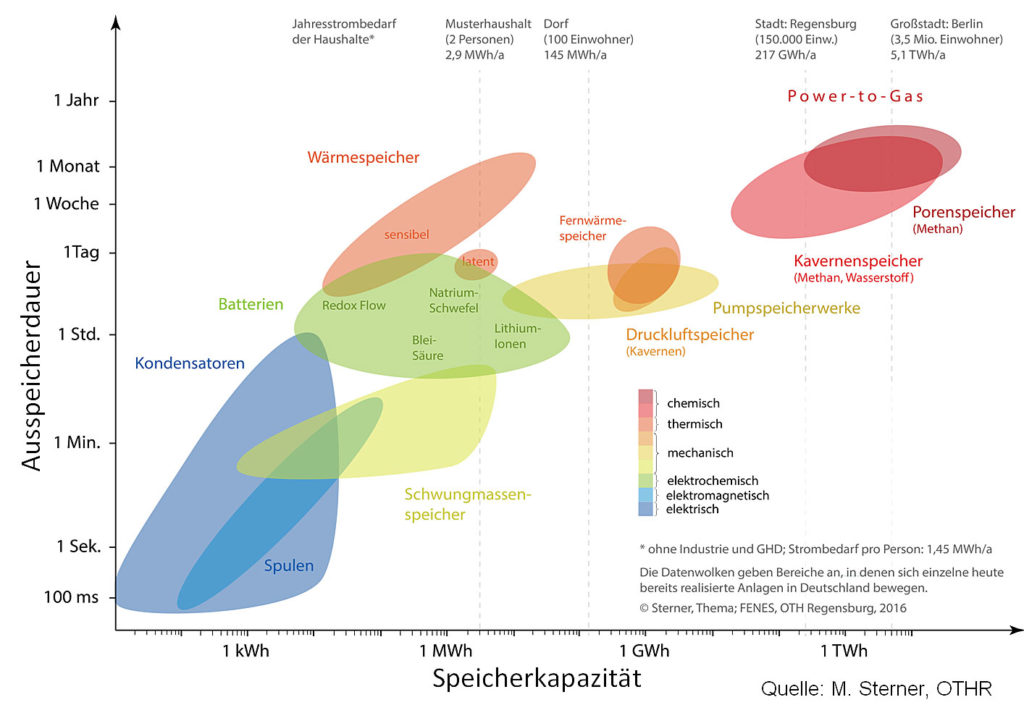
\includegraphics[width=0.6\paperwidth]{speicherkapazitaet.jpg}};
		\node[yshift=-2mm] at (T.south) {\tiny\citetitle{topler2019}~\parencite{topler2019}};
	\end{tikzpicture}
	\end{uncoverenv}
\end{frame}

\begin{frame}
	\frametitle{Hydrogen as a source of energy}
	\begin{tikzpicture}[overlay,remember picture]
		\node[anchor=north east,outer sep=2mm] at (current page.north east) {\scalebox{.5}{\usebox\stepcb}};
	\end{tikzpicture}
	\begin{itemize}
		\item Again, there are different methods to recover energy from hydrogen
		\item Fuel cells are the most common one
		\item In a fuel cell, hydrogen and oxygen react to produce electricity, heat, and water
		\item In this process, roughly 60\% of the energy is converted into
			electricity~\cite{tuv}
	\end{itemize}
\end{frame}

\section{Our roadmap}
\begin{frame}
	\frametitle{What hydrogen can do and what i can't}
	\begin{itemize}
		\item Let's try to calculate the overall efficiency\\\medskip
			$\text{Electrolysis} \rightarrow \text{Storing/Transportation} \rightarrow \text{Energy recovery}$\\
			$60\% \cdot 98\% \cdot 60\% = 35\%$\hfill\info{lower bound}\\
			$85\% \cdot \textcolor{gray}{\underbrace{\textcolor{black}{98\%}}_{\text{\clap{Hydrogen stored in salt caverns \cite{ees2022}}}}} \cdot 60\% = 50\%$\hfill\info{upper bound}\\\medskip
		\item Energy that's lost to heat can easily be used to heat buildings, thus
			increasing the efficiency
		\item But infrastructure gaps are still an unsolved problem
	\end{itemize}
\end{frame}

\section{References}
\begingroup
\defbibheading{bibliography}[\bibname]{}
\let\frametitle\oldft
\begin{frame}[allowframebreaks]
	\frametitle{References}
	\printbibliography
\end{frame}
\endgroup
\end{document}
